\chapter{Introducion} \label{ch:Introduction}
\section{Interferon-Induced Proteins with Tetratricopeptide Repeats} \label{sec:Interferon-Induced Proteins with Tetratricopeptide Repeats}
The interferon-induced proteins with tetratricopeptide repeats (\textit{IFIT}) gene family are interferon-stimulated genes (ISGs) that are activated early in antiviral response. In unstimulated cells, with the exception of some myeloid cell subsets, they are barely detectable; however, upon viral infection, their translated products become some of the most abundant proteins in the cell (\cite{Diamond2013TheProteins}). \textit{IFITs} are conserved in higher animals yet absent in the genomes of plants, insects, and yeast. 

With regards to their genomic composition, they are composed of two exons, the first encoding the ATG, two additional nucleotides and a 5' untranslated region (UTR), with the second exon containing the rest of the coding sequence and 3' UTR (\cite{deVeer1998IFI60/ISG60/IFIT4Genes}). Most of the IFIT family gene members contain multiple copies of specific sequences in their promoter regions called interferon-stimulated response elements (IRSE), which are targets for downstream effectors of the interferon signalling cascade, enabling the fast activation of IFIT gene transcription (\cite{Lou2009IFR-9/STAT2STAT1}).   

Most mammalian IFIT genes are categorised into 4 subgroups named IFIT1, IFIT2, IFIT3, and IFIT5 all with clear orthologous relationships (\cite{Sarkar2004NovelGenes}). Primates, along with some other mammalian species have a duplication of IFIT1 called IFIT1B, which lacks the ISRE in its gene promoter regions, and thus effectivelly only act as a pseudogene. Several rodents including mice and rats have lost the IFIT1 and IFIT5 genes and have duplications of IFIT1B and IFIT3 (\cite{Daugherty2016Evolution-guidedMammals.}) resulting in IFIT1B (typically referred to as IFIT1), IFIT1B-like gene 1, IFIT1B-like 2 gene, IFIT3 and IFIT3B genes. In contrast, avian species have lost most IFIT genes, with only one left resembling human IFIT5 (\cite{Liu2013Lineage-SpecificFamily}). These variations in IFIT gene numbers are most probably the result of differing evolutionary pressures posed by different viruses affecting their respective host species, although it is evident that maintaining IFIT genes in the genome must be beneficial. 

\subsection{Routes of \textit{IFIT} Expression Activation} \label{subsec:Routes of IFIT Expression Activation}
\subsubsection{Interferon Signalling} \label{Interferon Signalling}
\textit{IFIT} induction can be achieved by activating several arms of the innate immune system (Figure \ref{fig:Pathways Inducing ISG mRNA Production.}). The strongest inducers are type I interferons, such as Interferon alpha and beta (IFN\(\alpha\)/\(\beta\)).  Their signalling is mediated via activation of IFN\(\alpha\)/\(\beta\) receptor and the subsequent downstream Janus kinase (JAK), and Signal transducer and activator of transcription (STAT) signal transduction. As a result, interferon-stimulated gene factor 3 (ISGF3), consisting of phosphorylated STAT1 and STAT2 proteins bound to interferon regulatory factor (IRF) IRF9, translocates to the nucleus, binds to the ISRE in the IFIT promoters and induces their transcription (\cite{Der1998IdentificationArrays}; \cite{Mesev2019DecodingInfection}; \cite{Schoggins2011Interferon-stimulatedFunctions}). 

\subsubsection{Pattern Recognition Receptors} \label{Pattern Recognition Receptors}
Another arm of \textit{IFIT} activation is mediated through several pattern recognition receptors (PRRs), which can recognise various pathogen-associated molecular patterns (PAMPs). \textit{IFITs} have been reported to be induced by bacterial PAMPs such as lipopolysaccharide (LPS) from Neisseria meningitidis via activation of Toll-like receptor (TLR) 4 (\cite{Zhou2013InterferonDefense.}). Interestingly, TLR4 has also been observed to be activated by the glycoprotein of respiratory syncytial virus (RSV) (\cite{Funchal2015RespiratoryNeutrophils}). Other TLRs such as TLR3, TLR7, and TLR9 are capable of sensing PAMPs in the form of foreign nucleic acids in the endosomes. TLRs then interact with their adaptor proteins to in turn activate IRF3, IRF7, and nuclear factor kappa B (NF\(\kappa\)B), all of which have the capability to induce \textit{IFIT} family genes (\cite{Diamond2013TheProteins}). These pathways are often prevalent in lymphocytes, monocytes, and mast cells; however, cytosolic nucleic acid sensors are functional in a broader subset of cells (\cite{Ablasser2011WhereFit}).

\begin{figure}
    \centering
    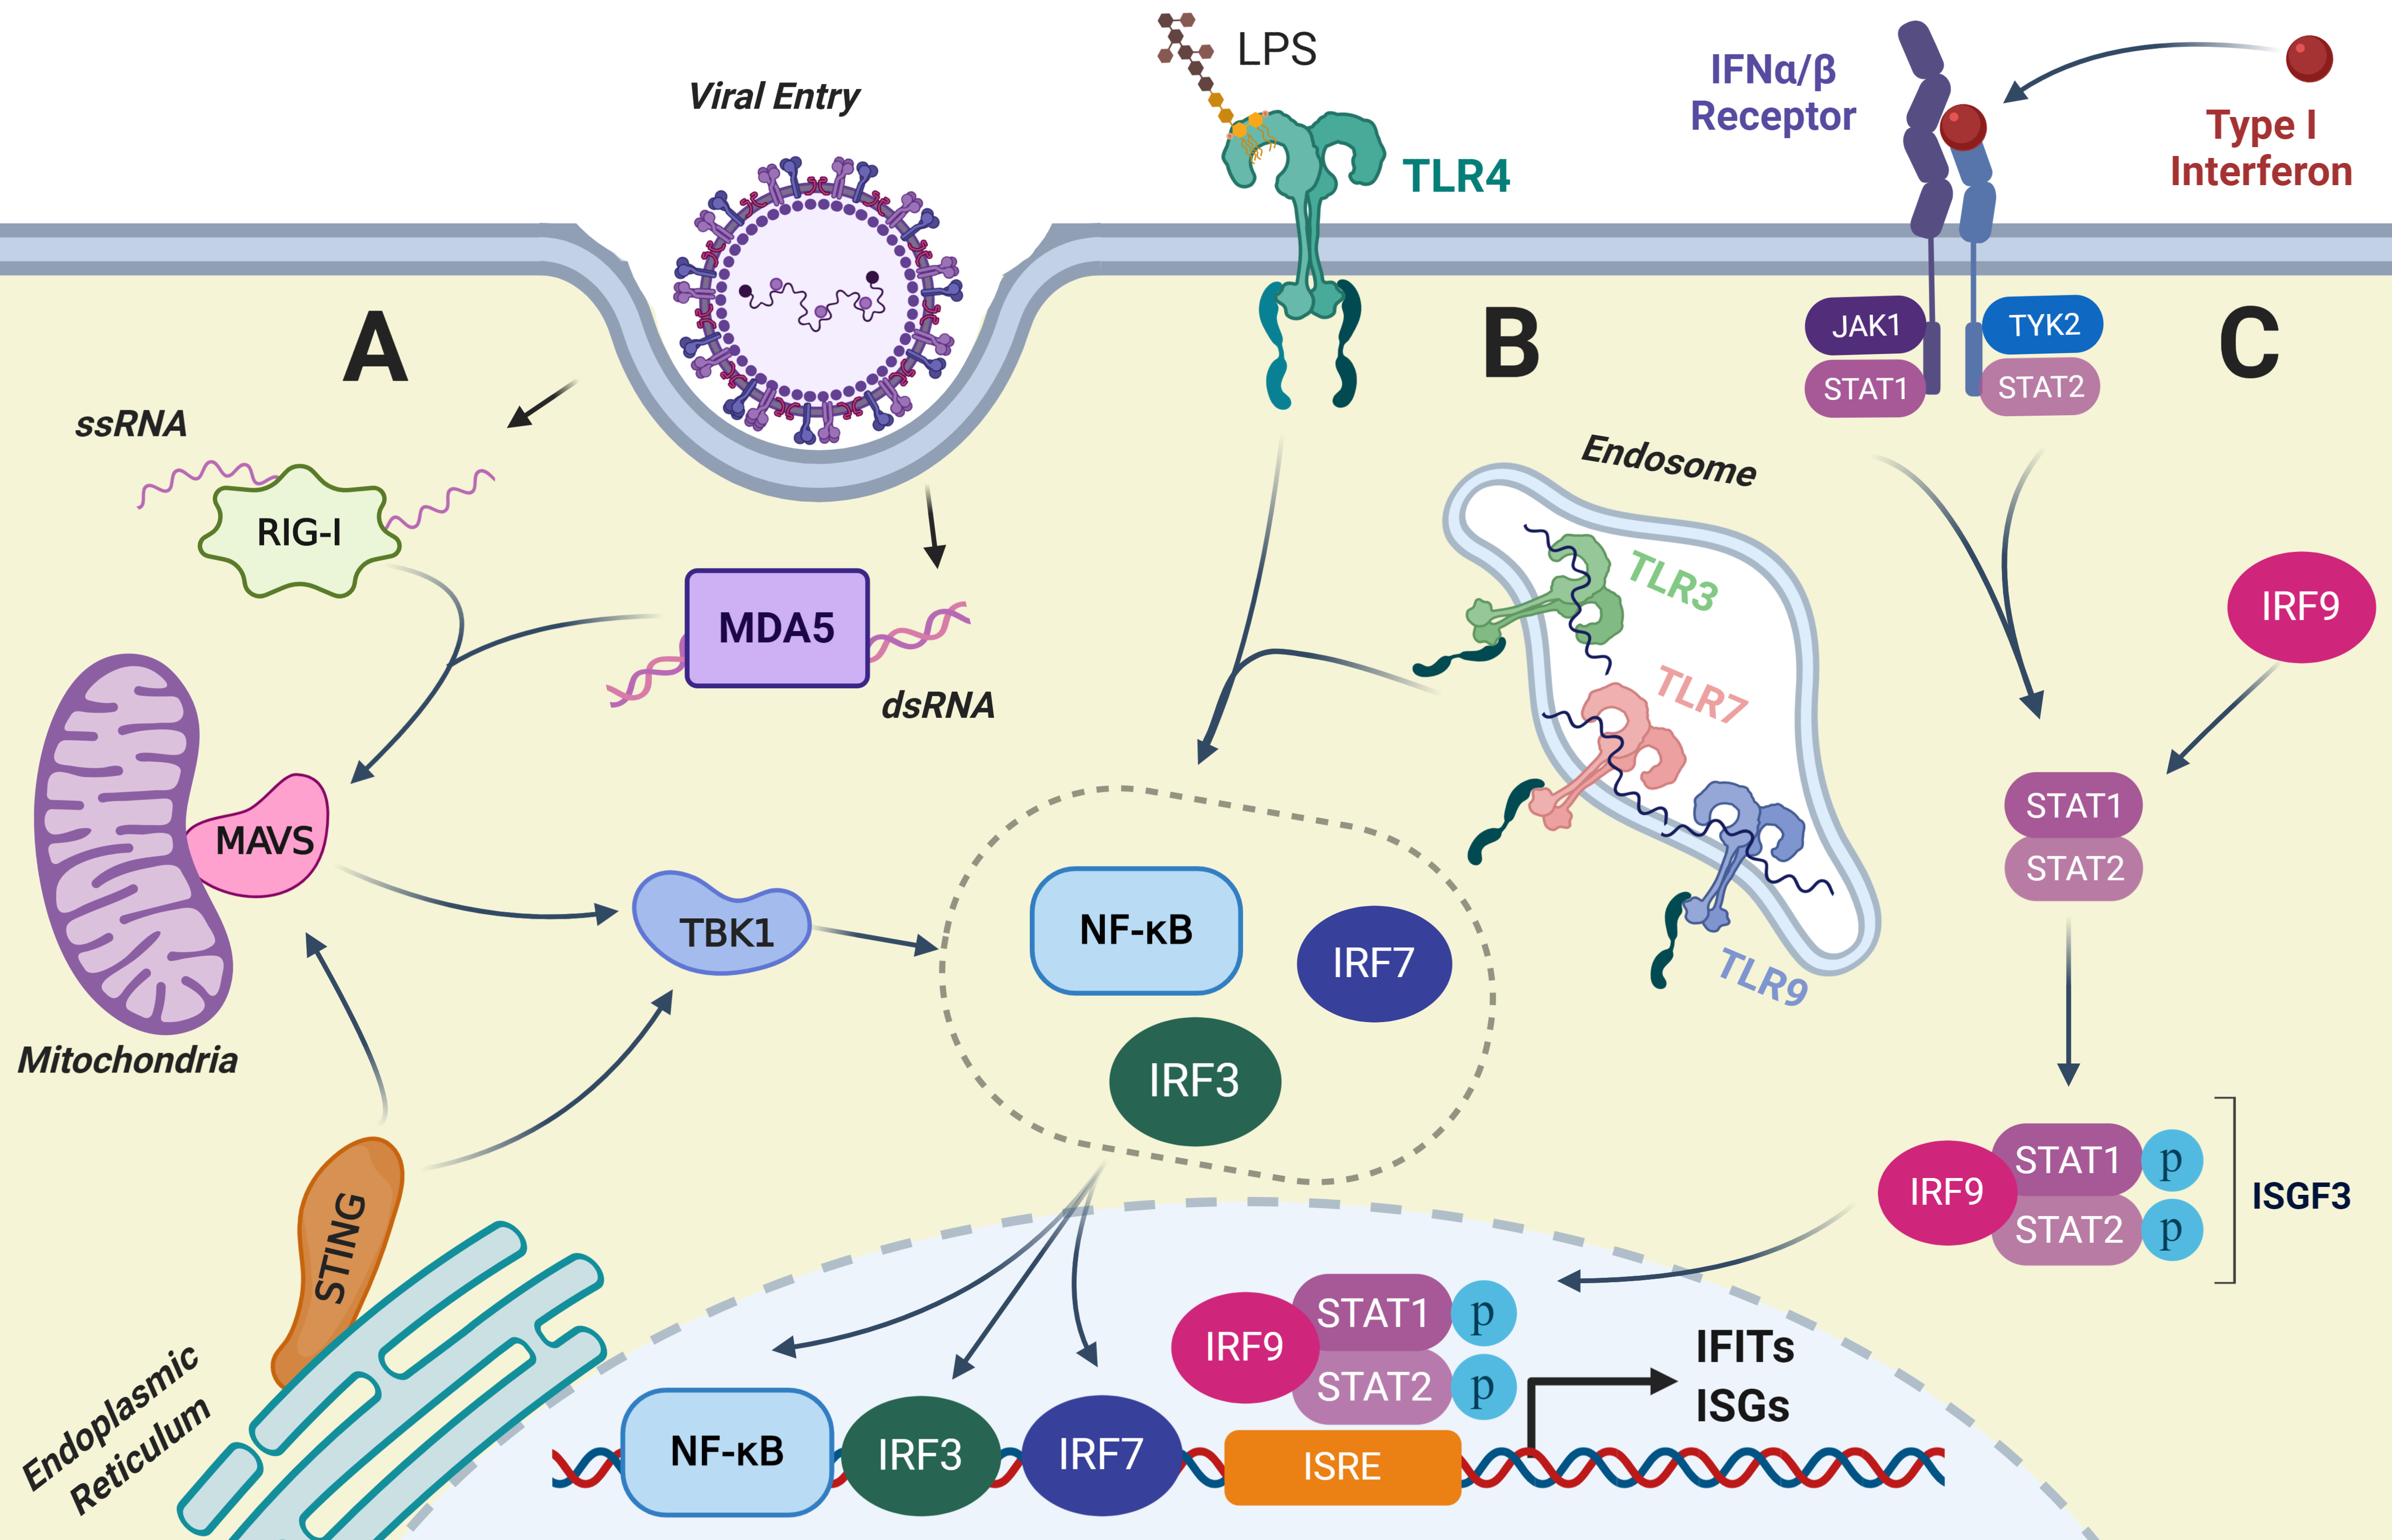
\includegraphics[width=1\linewidth]{04. Introduction//Figs/01. IFIT transcription activation figure.png}
    \caption[Pathways Inducing ISG mRNA Production.]{\textbf{Pathways Inducing ISG mRNA Production.} Three routes of ISGs transcription induction are depicted. Pathway A shows virus releasing its genome upon its entry and subsequent foreign nucleic acid detection by cytosolic sensors RIG-I and MDA5. These detect single-stranded and double-stranded RNA respectively. Both activate MAVS, which in turn activates TBK1. STING protein facilitates this activation by enhancing MAVS and TBK1 interaction. Pathway B shows PAMP detection by TLR receptors. TLR4 recognises LPS in the extracellular space while TLR3, TLR7, and TLR9 detect foreign nucleic acids in endosomes. TBK1, as well as TLR activation, leads to the translocation of activated IRF3, IRF7, and NF\(\kappa\)B into the nucleus where they promote ISGs transcription activation. Pathway C depicts type 1 interferon signalling pathway. IFN\(\alpha\)/\(\beta\) receptor activation leads to STAT1 and STAT2 activation. Further addition of IRF9 forms ISGF3 complex, which translocates into the nucleus onto ISRE and promotes ISGs transcription activation. ISG, interferon-stimulated genes; RIG-I, retinoic acid-inducible gene-I; MDA5, melanoma differentiation-associated gene 5; MAVS, mitochondrial antiviral signalling protein; TBK1, TANK-binding kinase 1; STING, stimulator of interferon genes; PAMP, pathogen-associated molecular pattern; TLR, toll-like receptor; IRF, interferon regulatory factor; NF\(\kappa\)B, nuclear factor kappa B; IFN, interferon; STAT, signal transducer and activator of transcription; ssRNA, single-stranded RNA; dsRNA, double-stranded RNA; ISGF, interferon-stimulated gene factor; ISRE, interferon-stimulated response elements. The figure was adapted from Diamond and Farzan, (2013) and Natalya Odoardi's BioRender template. Created with BioRender.com.}
    \label{fig:Pathways Inducing ISG mRNA Production.}
\end{figure}

\subsubsection{Cytosolic Nuclec Acid Sensors} \label{Cytosolic Nuclec Acid Sensors}
Cytosolic RNA sensors include melanoma differentiation-associated gene 5 (MDA5) and retinoic acid-inducible gene I (RIG-I) (\cite{Vladimer2014IFITs:Proteins}). Both signal through mitochondrial antiviral signalling protein (MAVS), which in turn activates IRF3, IRF7, and NF\(\kappa\)B as their downstream effectors (\cite{Ashley2019Interferon-IndependentCytomegalovirus}). In order to prevent activation by cellular RNA molecules, a precise RNA-recognition mechanism has to be conducted by the sensors. While MDA5 senses long double-stranded RNA (dsRNA) (\cite{Brisse2019ComparativeMDA5}), RIG-I is able to sense differences in the 5' RNA modifications (\cite{Schlee2016DiscriminatingSensing}). During mRNA maturation in higher eukaryotes, 7-methyl guanosine (m7G) is connected by a 5'- 5' triphosphate bridge, which is referred to as capping (\cite{Devarkar2016StructuralRIG-I}; \cite{Ramanathan2016MRNAApplications}). Several viruses carry uncapped, 5'-triphosphorylated (5'-PPP) or incompletely capped RNA (cap 0), whereas host animals possess cap-1 and cap-2 mRNA moieties (\cite{Choi2018ACaps}), which are all depicted in Figure \ref{fig:Overview of 5'RNA Modifications.}. \textit{IFITs} can be activated by several signal transduction pathways, each with its own inducers and kinetics. A cross-play of these pathways is what in turn orchestrates IFIT response during viral infection.

\begin{figure}
    \centering
    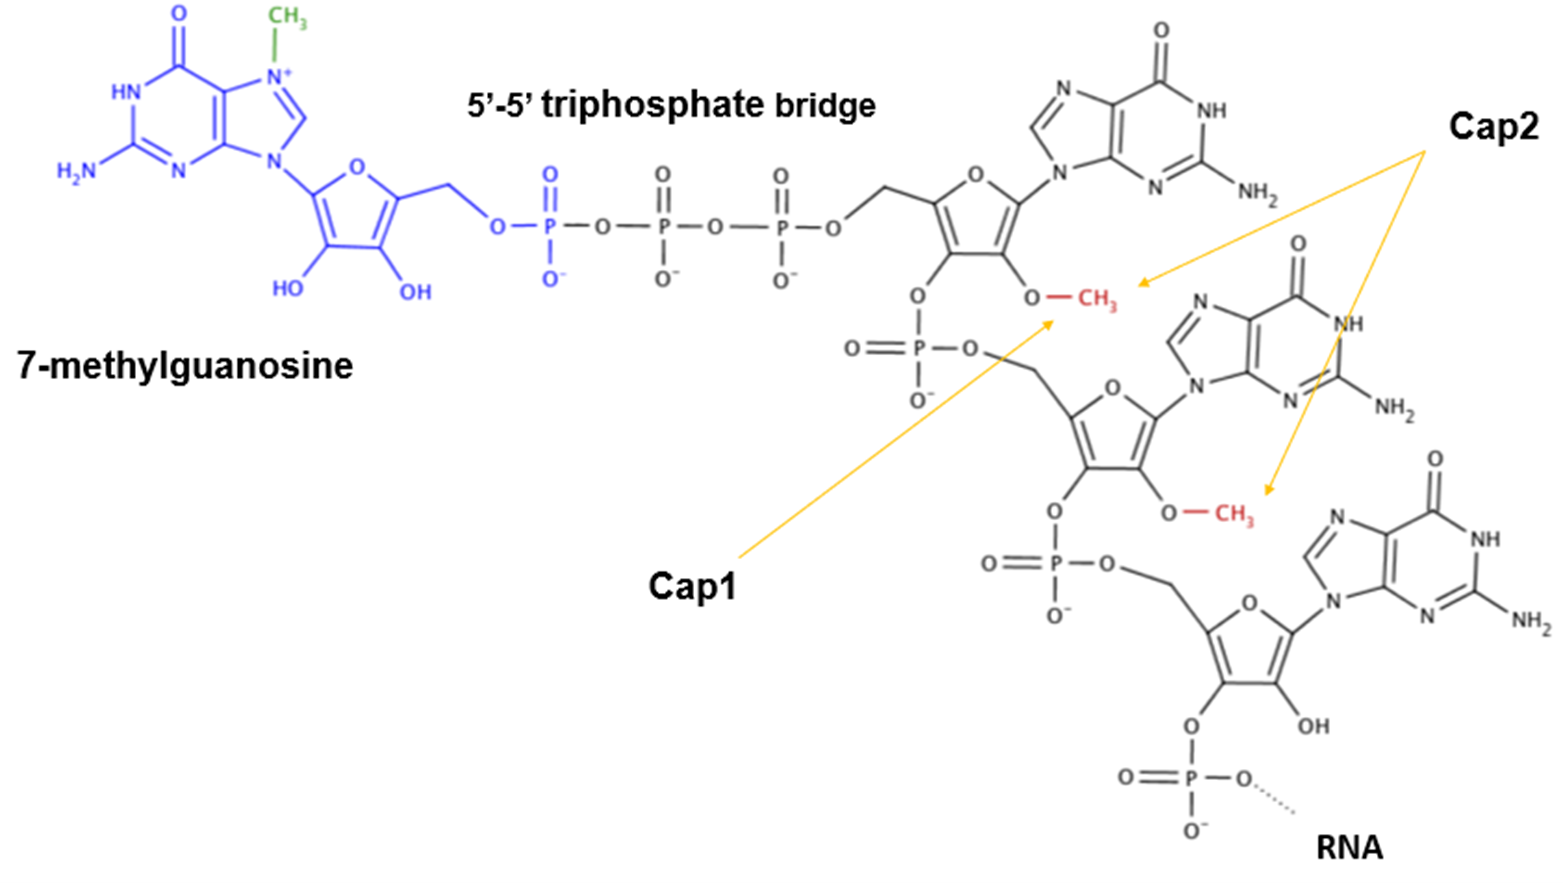
\includegraphics[width=0.75\linewidth]{04. Introduction//Figs/02. 5-RNA Modifications.png}
    \caption[Overview of 5'RNA Modifications.]{\textbf{Overview of 5'RNA Modifications.} Mature mRNA is displayed. Higher eukaryotes modify their mRNA by the initial addition of guanosine (blue) via 5' - 5' triphosphate bridge to the 5' end. Subsequently, the guanosine is methylated into 7-methylguanosine (green) and this modification is referred to as Cap0 structure. Furthermore, the first 2 bases of RNA can be methylated (red) and make either Cap1 or Cap2 structural modifications (yellow arrows). The figure was adapted from \cite{Picard-Jean2013RNAGenomes}.}
    \label{fig:Overview of 5'RNA Modifications.}
\end{figure}

\subsection{Structural Features of IFIT Proteins} \label{subsec:Structural Features of IFIT Proteins}
IFITs are composed of multiple copies of tetratricopeptide repeats (TPR). These are motifs comprised of 3-16 tandem repeats of 34 amino acids, which adopt helix-turn-helix confirmations (\cite{DAndrea2003TPRHelix}). TPRs are conserved in all species from bacteria through plants to higher animals and are commonly found in scaffolding proteins (\cite{Vladimer2014IFITs:Proteins}). IFIT TPRs are comprised of degenerate sequences meaning the conservation of the motif is limited. This allows different IFIT proteins to have a broader profile of protein interactors while still maintaining the overall conformation (\cite{Fensterl2015Interferon-InducedPathogenesis}). IFIT proteins are often subjected to post-translational modifications such as ubiquitination or ISGylation (addition of small IFN-induced ubiquitin-like proteins), which may alter IFIT stability and function.

\subsubsection{IFITs and Their Interaction with RNA} \label{IFITs and Their Interaction with RNA}
IFIT1 and IFIT5 both form a positively charged channel with an affinity for 5' ends of single-stranded RNA (ssRNA) molecules in a sequence non-specific manner. IFIT5 can accommodate 5'PPP RNA and effectively acts as a sensor for these molecules (\cite{Abbas2013StructuralProteins}; \cite{Pichlmair2011IFIT1RNA}). On the other hand, IFIT1 can accommodate m7G, but certain residues inside its channel prevent efficient binding of cap1 and cap2 moieties (\cite{Diamond2014IFIT1:Translation}; \cite{Mears2018BetterResponse}). Through these interactions they can effectively discriminate between self and non-self RNA moieties. IFIT2 is also capable of RNA binding, albeit independent on the 5'-capping state. The C terminals of IFIT2 homo-dimer create a super-helical structure with a positively-charged nucleotide-binding channel on its inner surface, which was observed to bind to AU-rich RNA molecules (\cite{Yang2012CrystalMechanisms}). Mechanistic studies identified IFIT2 binding to mRNAs as important to prevent ribosomal pausing and thus increasing the transnational efficiency of IFIT2-bound mRNAs, a process which has been observed to be hijacked by influenza A virus (\cite{Tran2020InfluenzaMRNAs}).

\subsubsection{Formation of IFIT Protein Complexes} \label{Formation of IFIT Protein Complexes}
As shown in Figure \ref{fig:IFIT Structures and Multimer Formation.}, all IFIT proteins, apart from IFIT5, can form homo- and hetero- dimeric and trimeric complexes. IFIT1 homodimerizes via its C-terminal domain (\cite{Abbas2013StructuralProteins}). The same domain has been shown to interact with the C termini of both IFIT2 and IFIT3, although the IFIT1:IFIT3 complex is more thermodynamically stable (\cite{Fleith2018IFIT3RNA}). Compared to IFIT1, IFIT5 has its dimerization motif shielded by its C terminal TPR and thus stays monomeric in solution (\cite{Kumar2014InhibitionMRNAs}). In contrast, IFIT2 and IFIT3 are rarely seen as monomeric in solution and rather stay as their respective homodimers or IFIT2:3 heterodimers. This is predicted to be done by swapping the third TRP domain in their N-terminal domains (Figure \ref{fig:IFIT Structures and Multimer Formation.}), which keeps them in a more thermodynamically stable configuration (\cite{Yang2012CrystalMechanisms}). IFIT2 homodimer forms a large positively charged cavity which has a propensity to bind dsRNA and AU-rich RNA molecules (\cite{Vladimer2014IFITs:Proteins}; \cite{Yang2012CrystalMechanisms}). IFIT3 interacts with IFIT1 via its C-terminal domain and this interaction increases the half-life of IFIT1 and its specificity for cap0 RNA. Thus, IFIT3 acts as an enhancer of IFIT1 action (\cite{Fleith2018IFIT3RNA}; \cite{Johnson2018HumanStability}). Recently, it has been shown that IFIT1, IFIT2, and IFIT3 form a heterotrimer, although the precise function of this complex has yet to be elucidated (\cite{Fleith2018IFIT3RNA}). In summary, TPR motifs allow IFITs to have a multitude of possible interaction partners, including themselves. Formation of IFIT homo- and hetero-oligomers influences their function and half-life, allowing for variable possible outcomes to occur following IFIT protein production based on the level of each of the proteins. 

\begin{figure}
    \centering
    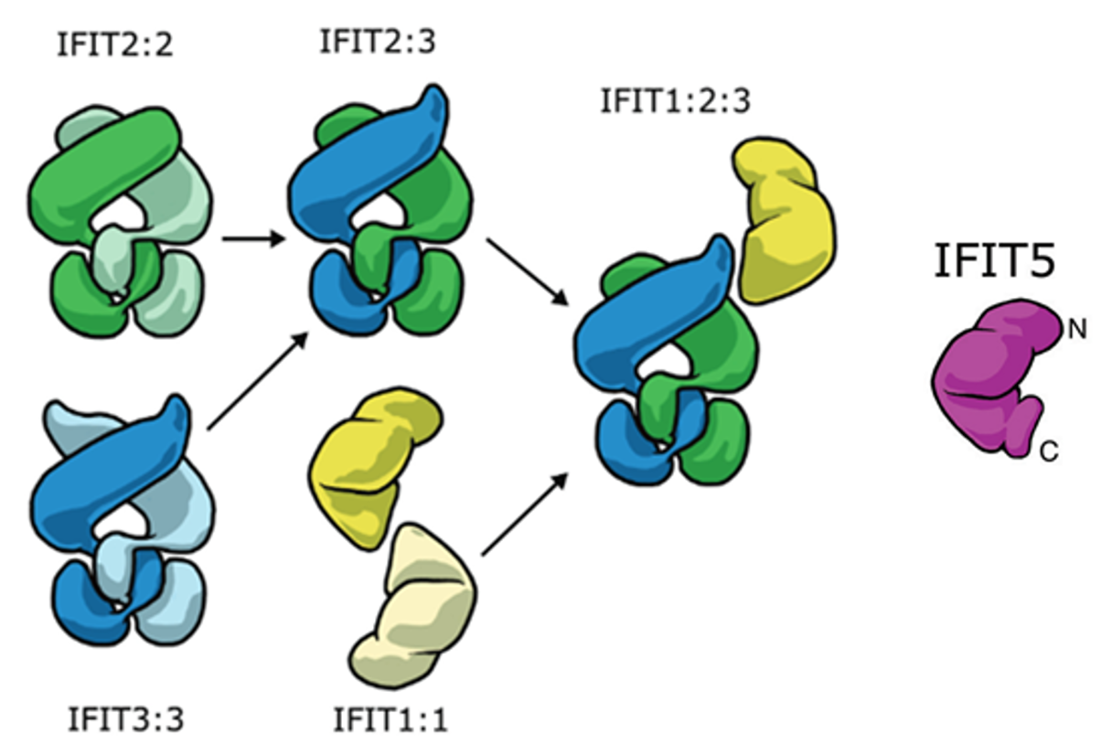
\includegraphics[width=0.75\linewidth]{04. Introduction//Figs/05. IFIT-complexes.png}
    \caption[IFIT Structures and Multimer Formation.]{\textbf{IFIT Structures and Multimer Formation.} IFIT tertiary and quaternary protein conformations are illustrated. IFIT1 is shown in yellow, IFIT2 in green, IFIT3 in blue, and IFIT5 is highlighted in purple. IFIT1 is able to homodimerise or heterooligomerise with IFIT2 and IFIT3 via its C terminal domain. IFIT5 has the corresponding interaction domain occluded by a helix and thus does not interact with the rest of IFIT proteins. IFIT2 and IFIT3 are capable of forming homodimers or heterodimers by ‘swapping’ TPRs in their N terminal regions. By combining the interactions IFIT1:2:3 heterotrimer is formed. The figure was adapted from \cite{Mears2018BetterResponse}.}
    \label{fig:IFIT Structures and Multimer Formation.}
\end{figure}

\subsection{Localisation and Functions of IFIT Proteins} \label{subsec:Localisation and Functions of IFIT Proteins}
\subsubsection{Localisation of IFIT Proteins} \label{Localisation of IFIT Proteins}
To date, IFIT protein localisation has been has been well studied in human and mouse models. Most publications indicate IFITs to be predominantly cytoplasmic. In more detail, nascent murine Ifit1 and human IFIT1 have been observed to localise diffusely in the cytoplasm while being excluded from the nucleus in NIH3T3 and P2.1 cell lines respectively (\cite{Pichlmair2011IFIT1RNA}; \cite{Terenzi2008Interferon-inducibleE1}). The human protein atlas, utilising two distinct anti-IFIT1 antibodies, indicates IFIT1 to have granular cytoplasmic and nuclear localisation in A431 and U2OS cells; and cytoplasmic, nuclear-excluded localisation in HeLa cells (\cite{Thul2017AProteome}). IFIT2 reported localisation in the literature yields inconsistent results. While nascent murine Ifit2 was observed to be cytoplasmic while also associated with the mitotic spindle in all phases of the cell cycle in NIH3T3 and B16F10 cell lines (\cite{Saha2006IdentificationProtein}), exogenously expressed human IFIT2 was reported to be cytosolic and thus excluded from mitochondria in HeLa cell line (\cite{Stawowczyk2011TheApoptosis}). The latter is in conflict with what the human protein atlas reports on a nascent IFIT2 localisation in HeLa and U2OS cell lines, wherein both report cytoplasmic vesicular localisation distribution (\cite{Thul2017AProteome}). IFIT3 has been indicated to localise cytoplasmically, with the evidence arising from exogenous overexpression experiments in THP-1 and HEK293T cells, with the latter further confirming IFIT3 colocalizing with mitochondria (\cite{Huang2008Interferon-inducedCells}; \cite{Liu2011IFN-InducedTBK1}). The human protein atlas confirms these findings by reporting nascent IFIT3 to show granular cytoplasmic localisation with partial nuclear staining in A431 and HeLa cell lines (\cite{Thul2017AProteome}). Lastly, there is a discrepancy with regard to IFIT5 subcellular localisation. While exogenously expressed IFIT5 has been observed to localise at the ruffled membrane at the cell surface and to colocalise with actin-rich protrusions from the apical cell surface in both fibroblast-derived WI-38 VA-13 and hepatocyte-derived Huh7 cell lines (\cite{Katibah2013TRNAIFIT5}), the human protein atlas reports nascent IFIT5 display granular cytoplasmic localisation with partial nuclear localisation and concentrations resembling the Golgi apparatus in A431 and SK-MEL-30 cell lines (\cite{Thul2017AProteome}). 

\subsubsection{Inhibition of Translation and Viral Replication} \label{Inhibition of Translation and Viral Replication}
IFITs can restrict viral replication by several mechanisms. IFIT1 and IFIT5 can physically prevent non-self RNA from interacting with eukaryotic initiation factor (eIF) 4F (\cite{Kumar2014InhibitionMRNAs}). IFIT1 and 2 block the binding of eIF3 to the eIF2-GTP-Met-tRNA ternary complex by interacting with the eIF3E subunit, whereas human IFIT2, and mouse IFIT1 and IFIT2, can block the formation of the 43S-mRNA complex by binding to the eIF3C subunit (\cite{Diamond2014IFIT1:Translation}; \cite{Guo2000CharacterizationVirus}). This is a cap-independent mechanism for viral translation inhibition, however, extensive IFIT expression can negatively influence the whole cellular translation processes via this mechanism and can hinder normal inflammatory responses. Overexpression of IFIT1 in human embryonic kidney (HEK) 293T cells inhibited the activation of IRF3 and NF\(\kappa\)B and the transcription of IFN\(\beta\) in response to polyinosinic-polycytidylic acid (poly I:C) (\cite{Li2009ISG56Response}). The previously mentioned affinity of IFIT2 for AU-rich RNA can also regulate cellular translation as a lot of transcripts for cytokines or apoptotic factors are rich in adenine and uracil (\cite{Palanisamy2012ControlMicroRNAs}). 

\subsubsection{Modulation of Innate Immune Response Signalling} \label{Modulation of Innate Immune Response Signalling}
IFIT proteins also have the potential to influence innate immune responses by direct interaction with signalling cascade proteins. IFIT3 can potentiate RIG-I signalling by forming a scaffold between MAVS and TANK-binding kinase 1 (TBK1), (\cite{Liu2011IFN-InducedTBK1}), whereas IFIT5 enhances this pathway upstream by recruiting RIG-I to MAVS (\cite{Zhang2013IFIT5Pathways}). IFIT5 has also been reported to help facilitate NF\(\kappa\)B activation via scaffolding its activation kinases (\cite{Zhang2013IFIT5Pathways}). On the other hand, studies show that IFIT1 can both negatively and positively influence RIG-I signalling, upstream of MAVS. IFIT1 interacts with the stimulator of interferon genes (STING), an enhancer of MAVS and TBK1 interaction and it was proposed that these conflicting actions are caused by its multiple binding sites on STING (\cite{Li2009ISG56Response}; \cite{Reynaud2015IFIT1Interferon}). 

\subsubsection{Effects on Cell Cycle Progression and Apoptosis} \label{Effects on Cell Cycle Progression and Apoptosis}
IFIT2 and IFIT3 also have roles in cellular homeostasis. IFIT2 overexpression induces the mitochondrial dependent apoptotic pathway. IFIT2 has been shown to localise on mitochondrial membranes and to directly interact with pro-apoptotic factors which lead to apoptosome formation and subsequent caspase-9 activation (\cite{Chen2017InhibitionApoptosis}; \cite{Diamond2013TheProteins}). Expression of IFIT3 has been observed to alleviate these effects, most probably by the formation of IFIT2:3 dimers (\cite{Mears2018BetterResponse}; \cite{Stawowczyk2011TheApoptosis}). IFIT3 has also been observed to have negative effects on proliferation via indirect degradation of cyclin-dependant kinase inhibitor p27. As a result, cell cycle progression halts at the G1/S transition checkpoint (\cite{Xiao2006RIG-GProteins}). An overview of the IFIT mechanisms of action is depicted in Figure \ref{fig:Overview of IFIT Mechanisms of Action}.

Therefore, IFITs not only act as complementary RNA sensors to RIG-I but are also important as mediators of a plethora of other processes. These range from regulation of transcription, activation and inhibition of innate immune signalling, and regulation of cell life cycle. It is again possible that preference for these actions is influenced by the levels of particular IFIT proteins and their interplay. Taking into consideration the above-described modes of IFIT expression activation, we can speculate that different stimuli such as viruses or signalling molecules at different concentrations will result in quite diverging actions of IFIT proteins on the phenotype of the cell.

\begin{figure}
    \centering
    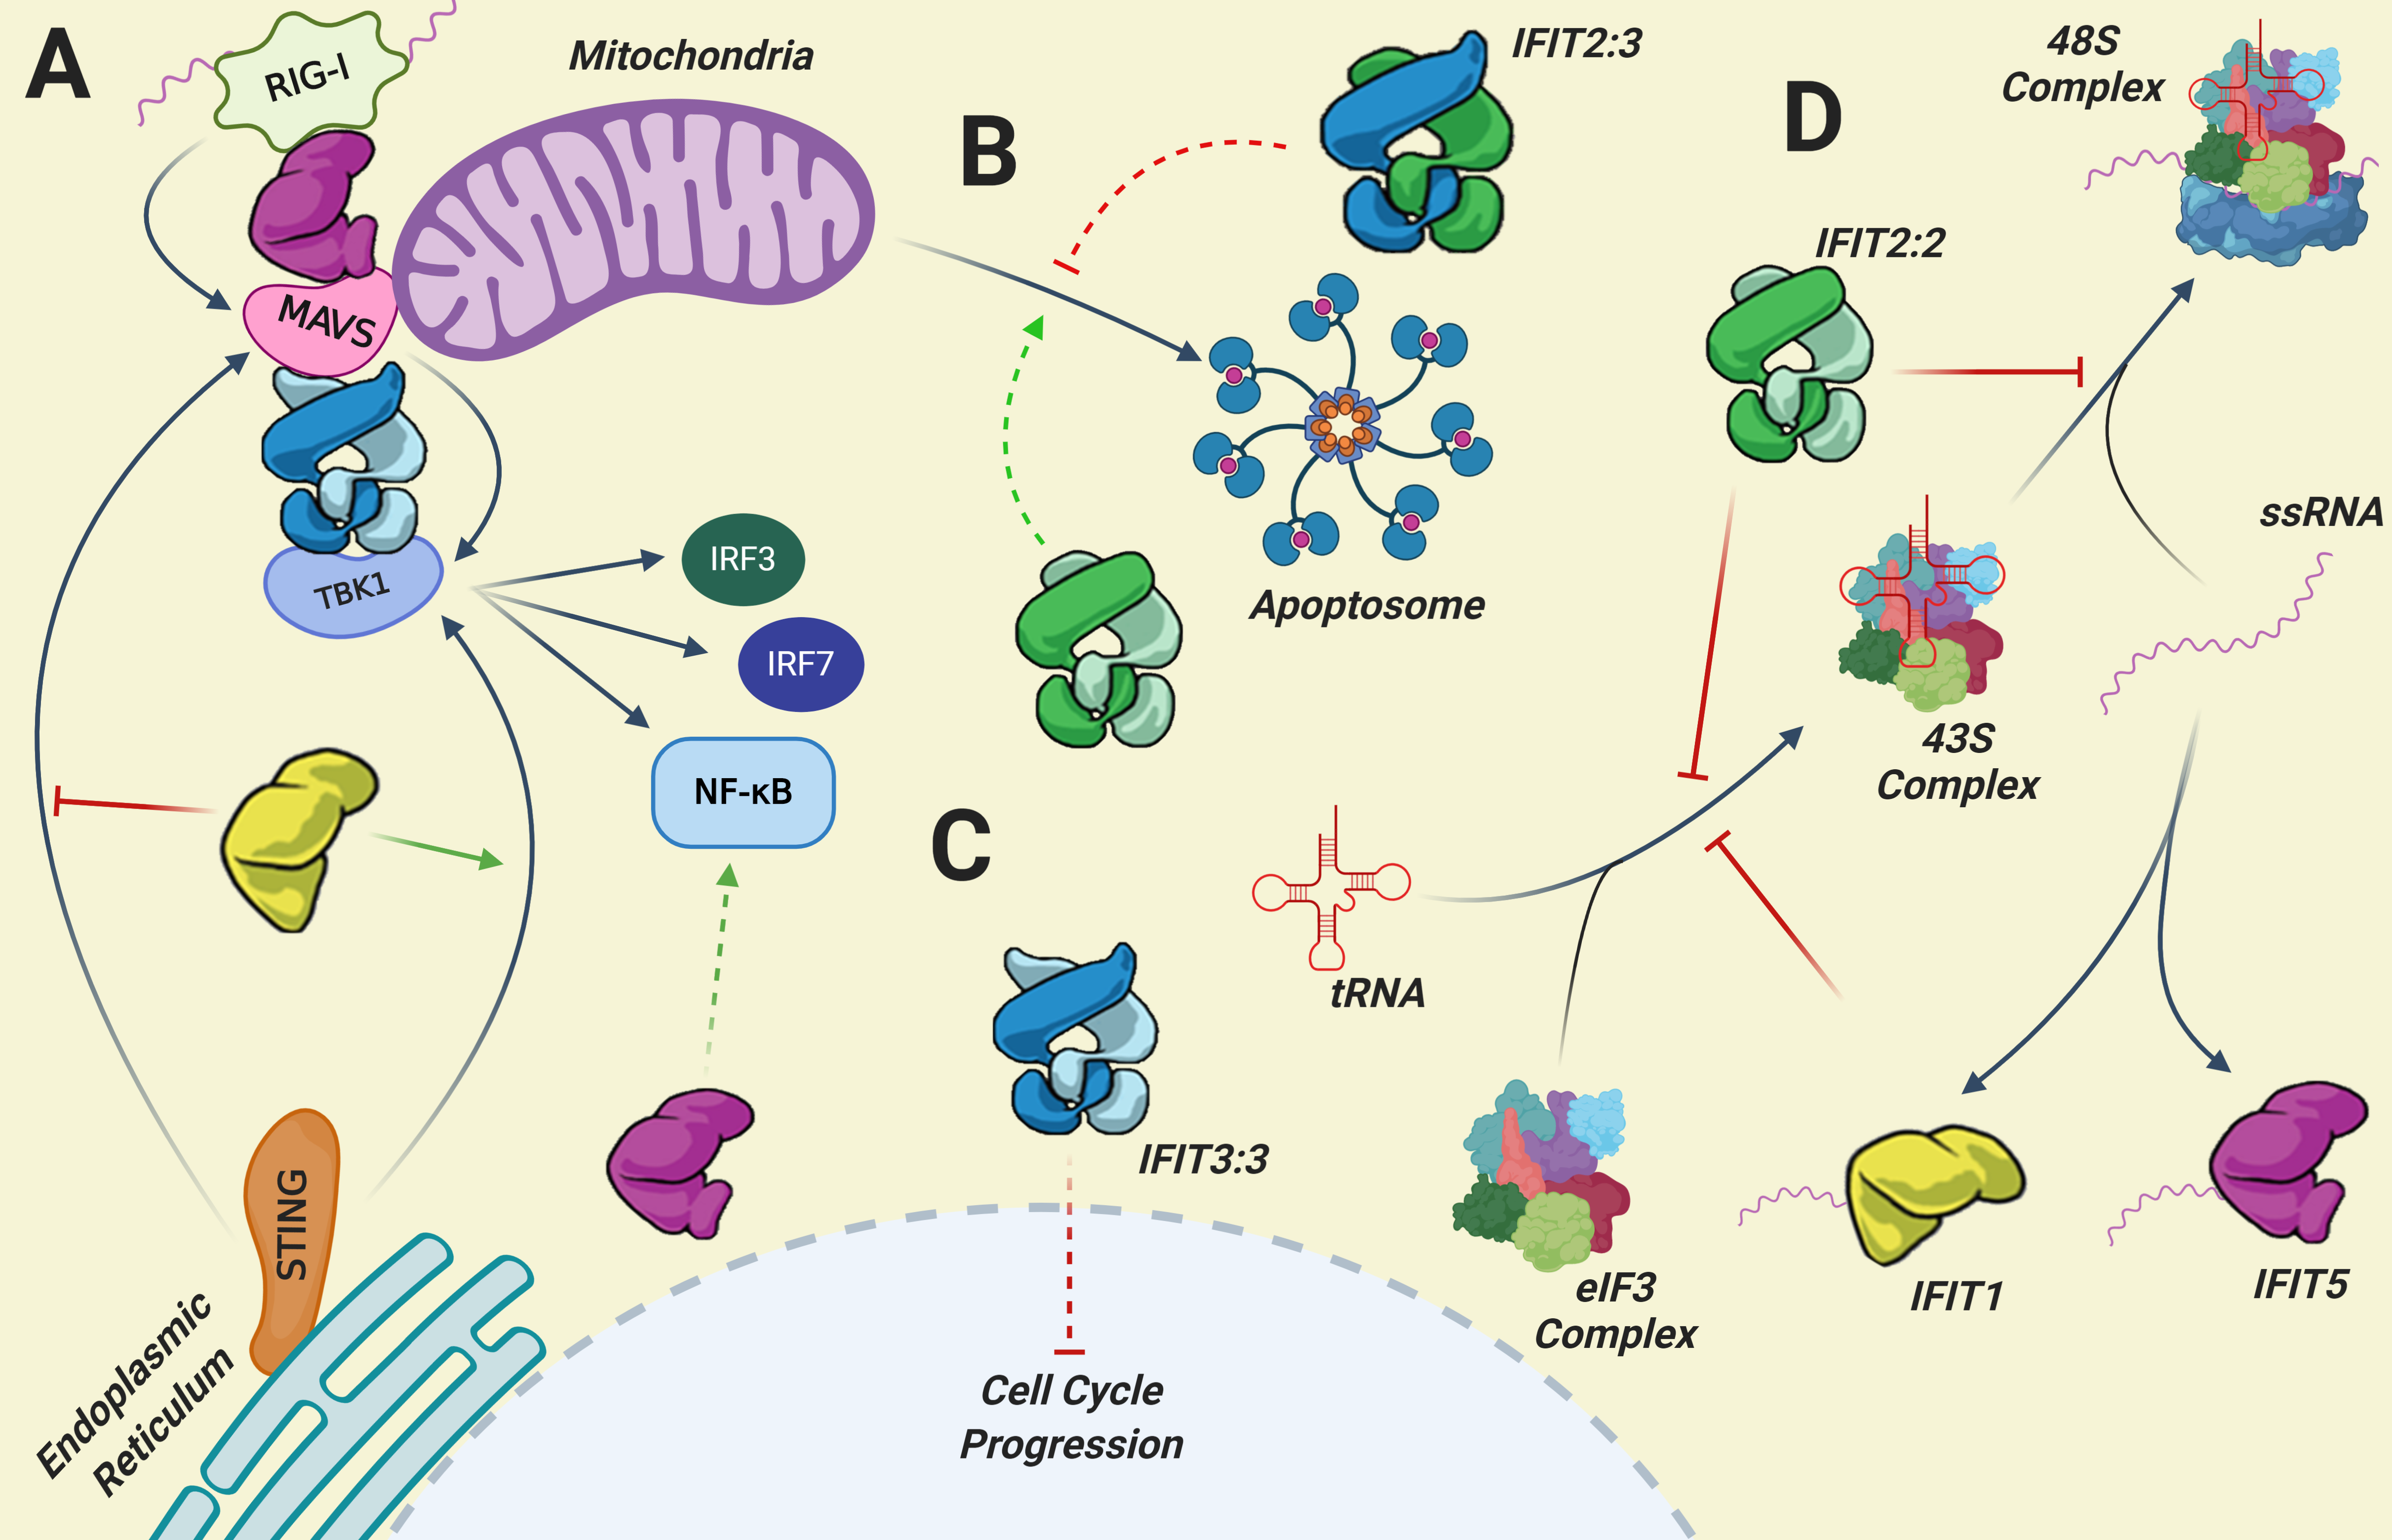
\includegraphics[width=1\linewidth]{04. Introduction//Figs/06. IFIT Mechanism of Action.png}
    \caption[Overview of IFIT Mechanisms of Action.]{\textbf{Overview of IFIT Mechanisms of Action.} IFITs have been described to have multiple actions in cells. Pathway A shows their involvement in innate immune signalling modulation. IFIT5 potentiate RIG-I activation of MAVS by scaffolding the two proteins together. IFIT3:3 further scaffolds MAVS to its effector, TBK1, which induces IRF3, IRF7 and NF\(\kappa\)B nuclear translocation when activated. STING protein also potentiates MAVS and TBK1 interaction. IFIT1 has been observed to inhibit STING interaction with MAVS while potentiating its interaction with TBK1. IFIT5 can also indirectly activate NF\(\kappa\)B. Pathway B shows IFIT2:2 involvement with apoptosome formation. IFIT2:3 complex reduces the pro-apoptotic activity of IFIT2:2. IFIT3:3 is involved in cell cycle arrest, as depicted in pathway C. Pathway D shows IFIT inhibition of viral replication and cellular translation. IFIT1 and IFIT5 can directly bind to cap0 and 5’PPP mRNA respectively and prevent its translation. IFIT1 and IFIT2 can both prevent 43S complex formation, while IFIT2 can also inhibit 48S complex formation. IFIT, Interferon-Induced Protein with Tetratricopeptide Repeats; RIG-I, retinoic acid-inducible gene I; MAVS, mitochondrial antiviral signalling protein; TBK1, TANK-binding kinase 1; STING, stimulator of interferon genes; IRF, interferon regulatory factor; NF\(\kappa\)B, nuclear factor kappa B; eIF, eukaryotic elongation factor; ssRNA, single-stranded RNA; tRNA, transfer RNA. The figure was adapted from \cite{Mears2018BetterResponse} and \cite{Diamond2013TheProteins}. Created using BioRender.com.}
    \label{fig:Overview of IFIT Mechanisms of Action}
\end{figure}

\subsection{IFIT Responses to Viral Infections} \label{subsec:IFIT Responses to Viral Infections}
Human IFIT effects on single-stranded RNA viruses have been studied extensively within the past decade. \cite{Rabbani2016Identification3} reported that IFIT1 and IFIT3 restrict human parainfluenza virus 3 (PIV3, negative-sense ssRNA virus), while ectopic expression of IFIT2 and IFIT5 did not affect the viral fitness. \textit{In vitro} IFIT1 knock-down experiments using short hairpin RNA showed marked enhancement of protein expression of human PIV2, PIV5, and mumps virus, all negative-sense ssRNA viruses (\cite{Andrejeva2013ISG56/IFIT1Synthesis}; \cite{Young2016HumanFamily}). Hantaviruses, a family of negative-sense ssRNA viruses such as Prospect Hill virus (PHV), and Tula virus (TULV), strongly induce IFIT3 expression during the course of their infection (\cite{Matthys2011TheInduction}). Most importantly within the non-segmented negative-sense ssRNA viruses, IFIT1, IFIT2, and IFIT3 have been reported to be globally antiviral against respiratory syncytial virus (RSV). Dori and colleagues either overexpressed or silenced these 3 IFITs and assessed RSV fitness by quantifying the viral mRNA produced. They reported decreased viral fitness following overexpression, while silencing of IFITs increased the viral mRNA production (\cite{Drori2020InfluenzaProteins}). Another negative-sense ssRNA virus, which bears a segmented genome, influenza A virus, has been shown to upregulate IFIT1, IFIT2, and IFIT3 in primary macrophages during infection (\cite{Lietzen2011QuantitativeMacrophages}). Recent studies also show the ability of IFIT1 and IFIT2 to negatively influence the viral fitness of influenza, as the knock-down of these IFITs resulted in increased viral RNA and protein production, while the opposite was true if IFIT1 and IFIT2 were overexpressed (\cite{Zhu2023TheSynthesis}). Human IFIT1 has been observed to be differentially expressed during hepatitis C virus (HCV) infection. HCV was described to suppress IFIT1 upregulation and subsequent experiments showed an inverse relationship between artificial levels of IFIT1 and HCV ability to infect host cells (\cite{Raychoudhuri2011ISG56Replication}, \cite{Ishida2019HepaticInfection}). Currently, there is very limited information about the effect of bovine IFIT expression on the viral fitness of bovine viruses.


\section{Respiratory Syncytial Virus} \label{sec:Respiratory Syncytial Virus}
Human and bovine Respiratory Syncytial Viruses (hRSV and bRSV) are enveloped, negative-sense, single-stranded RNA viruses belonging to the Orthopneumovirus genus (\cite{Afonso2016Taxonomy2016}). These viruses are recognized for inducing acute respiratory disease, which is confined to their respective hosts. Despite this host specificity, shared genetic and antigenic characteristics are observed among these closely related viruses (\cite{Buchholz2000ChimericVaccine}). hRSV primarily infects humans, while bRSV infects cattle. They are known to be the leading causes of lower respiratory tract illness in their respective hosts (\cite{Nair2013GlobalAnalysis}; \cite{Sacco2014RespiratoryCattle}). Although these viruses can infect individuals of all ages, severe respiratory illness, including bronchiolitis and pneumonia, is more common in infants, the elderly, and immunocompromised individuals (\cite{Falsey2005RespiratoryAdults}; \cite{Coultas2019RespiratoryAge}). On a global scale, hRSV affects nearly all children by the age of five, resulting in approximately 35 million cases and 3.5 million hospital admissions annually in the United States of America (\cite{Shi2017GlobalStudy}). Tragically, around 60,000 hospitalized children under the age of five succumb to the infection, with a notably higher mortality rate among infants under six months, especially those at high risk due to factors such as premature birth and pre-existing chronic lung and heart conditions (\cite{Shi2017GlobalStudy}; \cite{Jha2016RespiratoryVirus}; \cite{Coultas2019RespiratoryAge}). Bovine RSV infection also poses a significant threat to the global cattle farming industry, resulting in substantial economic losses (\cite{Brodersen2010BovineVirus}; \cite{Valarcher2007BovineInfection}).

Despite extensive research and development efforts spanning several decades, the availability of approved vaccines against hRSV remains limited. Historical challenges include the failure of the formalin-inactivated RSV vaccine, which led to enhanced natural infection in some vaccinated children (\cite{Fulginiti1969RespiratoryVaccine.}; \cite{Kim1969RespiratoryVaccine.}). Additional hurdles involve the heterogeneity of RSV subtypes and the incomplete immune responses generated against the virus. However, recent advances in the field have introduced a range of vaccine strategies, including live-attenuated wild-type virus, vector-based, viral protein sub-unit, mRNA-based, and DNA-based candidates. Presently, 24 vaccines are in various stages of clinical development, including two licensed vaccines: Arexvy (GSK) and Abrysvo (Pfizer). These vaccines are used as immunizing agents to prevent lower respiratory tract disease in older adults, with Abrysvo additionally indicated for passive immunization of infants through maternal administration during pregnancy (\cite{Topalidou2023RespiratoryVaccines}). In contrast, there are several vaccines available for bRSV, with the first one dating back to the 1970s. However, these vaccines offer only mild protection. Consequently, there is a pressing need to develop more efficacious vaccines for both hRSV and bRSV (\cite{Ellis2017HowCattle}).

\subsection{Genomic and Virion Composition} \label{subsec:Genomic and Virion Composition}
The size of the RNA genome of human and bovine RSV is reported to be 15,223 nucleotides for hRSV A2 subtype and 15,140 nucleotides for bRSV A51908 subtype, as reported by GenBank (GenBank identifiers KT992094 and NC038272 respectively). The RSV genome contains ten genes in the order 3'-NS1-NS2-N-P-M-SH-G-F-M2-L-5' (Figure \ref{fig:The Composition of RSV Virion and Genome}, panel b), which are transcribed into 10 monocistronic, capped, methylated, and polyadenylated mRNAs (\cite{Collins2013RespiratoryDisease}; \cite{Bohmwald2016HumanPathology}). These encode for 11 proteins as \textit{M2} gene is composed of two overlapping open reading frames (ORFs), which are accessed by coupled translation, where the ribosomes translating the first ORF (M2-1) move a short distance upstream after termination and reinitiate translation from a second (M2-2) overlapping ORF (\cite{Gould2007Pneumovirinae}).

RSV virions were observed to be pleomorphic, confronting to spherical (circa 100 nm radius), asymmetric, and filamentous (circa 5 \(\mu\)m in length) structures, as observed by electron microscopy, with a conserved structural organisation (\cite{Kiss2014StructuralComplex}). Virions produced in cell culture are predominantly observed to be filamentous in several cell types leading to a hypothesis stating that the spherical and asymmetric particles are the breakdown and aggregation by-products of filamentous particles (\cite{Ke2018TheTomography}, \cite{Conley2022HelicalVirus}). Within an \textit{in vitro} context, a substantial portion (95\%) of the progeny virus persists attached to the cell surface, appearing as particles that have seemingly undergone incomplete budding. The standard procedure for cultivating virus stocks involves subjecting infected cells to processes such as sonication, freeze-thawing, or vortexing, aimed at detaching the virus. It is important to note, however, that these methods lead to a reduction in infectivity and an increase in the risk of cellular contamination (\cite{Collins2013RespiratoryDisease}).

A representative filamentous RSV virion, based on the current literature, is depicted in Figure \ref{fig:The Composition of RSV Virion and Genome}, panel a. It is composed of the structural proteins, which include F, G, SH, M, M2-1, N, P and L proteins. M2-1 (transcription processivity factor) and matrix (M) proteins form subsequent lattice structures which support the viral membrane and dictate the filamentous shape of the virion (\cite{Conley2022HelicalVirus}). The attachment (G) and fusion (F) glycoproteins are embedded in the viral membrane and helically ordered in pairs, as dictated by the M lattice. The small hydrophobic (SH) protein is also embedded in the membrane (\cite{Ke2018TheTomography}, \cite{Conley2022HelicalVirus}). Inside the virion resides nucleocapsid which is composed of RSV genomic RNA-bound within the groves nucleoprotein (N) multimeric protein complexes. These have been observed to be found in two forms, either as a polymer of helical nucleocapsid, which spans several RSV genomes in its structure (Figure \ref{fig:Nucleocapsid Polymer and Its Interaction with Viral RNA}; \cite{Tawar2009CrystalVirus}; \cite{Conley2022HelicalVirus}) or double-decameric N-RNA rings (\cite{Gonnin2023StructuralNucleocapsids}; \cite{Gonnin2022ImportanceVirus}; \cite{Conley2022HelicalVirus}). These further interact with the large polymerase subunit (L) and the phosphoprotein polymerase cofactor (P) to form the ribonucleoprotein complex (RNP) (\cite{Gonnin2023StructuralNucleocapsids}). The P stabilises the RNP structure with the virion by interacting with M2-1 protein (\cite{Mason2003InteractionActivity.}).

\begin{figure}
    \centering
    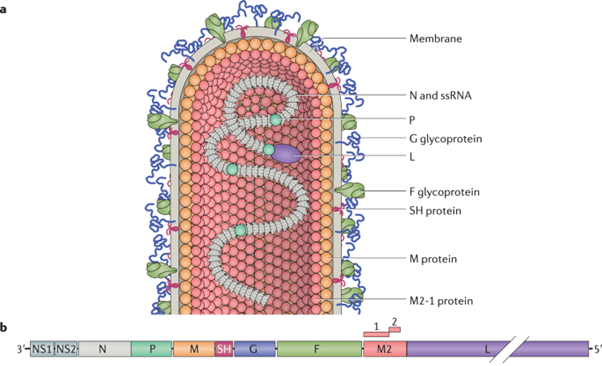
\includegraphics[width=1\linewidth]{04. Introduction//Figs/07. RSV-composition.png}
    \caption[The Composition of RSV Virion and Genome.]{\textbf{The Composition of RSV Virion and Genome.} a) The most biologically correct diagram of the filamentous RSV virion is depicted. M2-1 (transcription processivity factor) and matrix (M) proteins form subsequent lattice structures which support the viral membrane and dictate the filamentous shape of the virion. The attachment (G) and fusion (F) glycoproteins are embedded in the viral membrane and helically ordered in pairs, as dictated by the M lattice. The small hydrophobic (SH) protein is also embedded in the membrane. Inside the virion, a helical nucleocapsid is present, composed of viral RNA genome-bound nucleoprotein (N) polymer, with its precise protein structure shown in grey. The large polymerase subunit (L) and the phosphoprotein polymerase cofactor (P) are also associated with N. b) The human RSV genome from the A2 strain is shown to scale. it contains 10 genes encoding 11 proteins, with the M2 gene encoding the M2-1 and M2-2 proteins. ssRNA; single-stranded RNA. Figure taken from \cite{Battles2019RespiratoryIt} and the structural biology basis for this figure is from \cite{Conley2022HelicalVirus}.}
    \label{fig:The Composition of RSV Virion and Genome}
\end{figure}

\begin{figure}
    \centering
    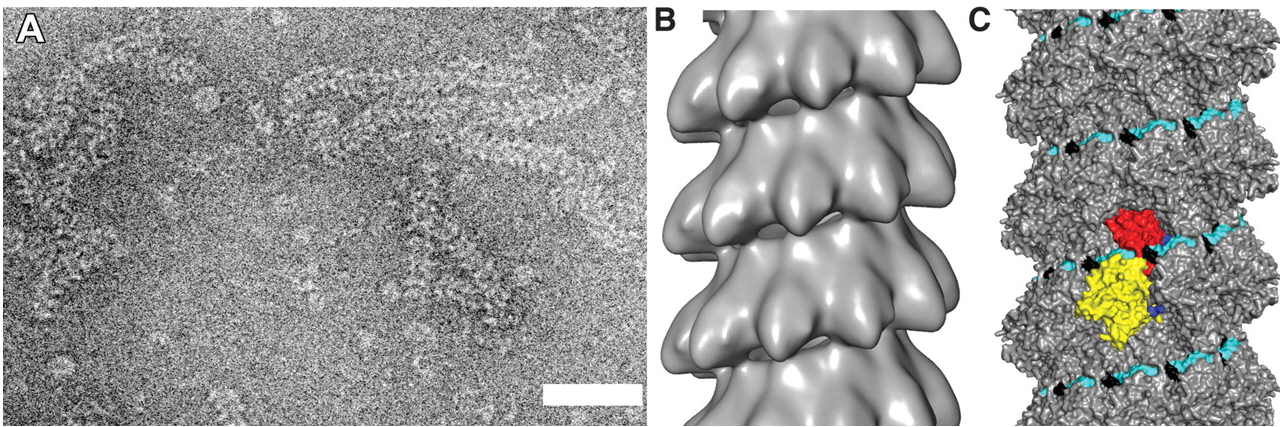
\includegraphics[width=1\linewidth]{04. Introduction//Figs/08. N-structure.jpeg}
    \caption[Nucleocapsid Polymer and Its Interaction with Viral RNA.]{\textbf{Nucleocapsid Polymer and Its Interaction with Viral RNA.} Panel A shows a negative-stained electron micrograph of recombinant RSV nucleocapsid-like helices. The scale bar indicates 50 nm. Panel B presents the 26 \r{A}-resolution 3D reconstruction of the observed helices formed by the nucleocapsid polymer. A single helix comprises 9.8 N subunits per turn. Panel C provides a more detailed view of the structure, with the encapsulated RNA shown in cyan and one N protein labelled based on its domains, with the N-terminal domain coloured in yellow and the C-terminal domain coloured in red. Figure adapted from \cite{Tawar2009CrystalVirus}.}
    \label{fig:Nucleocapsid Polymer and Its Interaction with Viral RNA}
\end{figure}

\subsection{RSV Protein Function and Viral Life Cycle} \label{subsec:RSV Protein Function and Viral Life Cycle}
Both F and G are the main antigenic proteins of RSV (\cite{Collins2011ProgressYears}). The F protein is involved in viral entry and assembly. It is generated as an inactive F0 precursor in the cytoplasm, after which it is activated by furin-like proteases in the Golgi apparatus (\cite{Collins1984NucleotideVirus}). The active form of the F protein in the viral particles is a trimer in a prefusion conformation (\cite{Ternette2007ImmunogenicityVirus}). The fusion protein has been reported to interact with several host surface receptors, such as toll-like receptor 4 (TLR4; \cite{Marr2012RoleReplication}), intercellular adhesion molecule-1 (ICAM-1; \cite{Behera2001BlockingInfection}), or nucleolin, with the latter believed to be the main RSV receptor and determinant of viral tropism (\cite{Tayyari2011IdentificationVirus}). 

The G protein is not vital for successful infection and is present in two forms, either as a membrane-bound form or a secreted isoform. Membrane-bound G enhances F protein binding to cellular surface receptors by facilitating membrane attachment via the interaction with heparin and annexin 2 (\cite{Collins2013RespiratoryDisease}; \cite{Krusat1997Heparin-dependentCells}; \cite{Malhotra2003IsolationCells}), while the secreted form is responsible for immune system evasion by antibody binding saturation (\cite{Bukreyev2008TheLeukocytes}). 

The transmembrane SH protein, situated as well at the virion surface, forms pentameric pore-like structures that exhibit cation-selective channel-like activity (\cite{Carter2010DirectPermeability.}, \cite{Gan2012TheChannels}). While the significance of this activity for RSV remains unclear, the SH protein is identified as a viroporin, belonging to a category of small viral proteins capable of modifying membrane permeability and influencing processes such as budding and apoptosis. Reports suggest that SH has a modest effect in reducing apoptosis via the interaction with B-cell receptor-associated protein 31 (BAP31), as documented by \cite{Fuentes2007FunctionProtein.}. Moreover, SH appears to inhibit signalling from TNF-\(\alpha\), an antiviral cytokine (\cite{Fuentes2007FunctionProtein.}). Recombinant RSV lacking SH demonstrates a somewhat more efficient \textit{in vitro} replication compared to the wild-type virus, possibly attributed to its smaller genome size and reduced number of genes. Additionally, this SH-deficient variant shows a slight attenuation in both mice and chimpanzees (\cite{Whitehead1999RecombinantChimpanzees}). It has been observed for \(\Delta\)SH RSV virus infection to result in enhanced tumour necrosis factor (TNF) signalling and increased production of IL-1\(\beta\), which could explain the observations mentioned above (\cite{Pollock2017ModulationProtein}). 

Along these lines, the non-structural proteins NS1 and NS2 main function seems to be the modulation of innate immune responses.

... about NSs \cite{Sedeyn2019RespiratoryResponses} - NSs
\cite{Pei2021Nuclear-localizedTranscription} - nuclear ns1 modulates host gene transcrition

While the two proteins can function separately, they appear to form complexes and may have synergistic effects, but this is poorly understood (Spann et al. 2005; Swedan et al. 2011). NS1 and NS2 interfere with innate immune responses including interferon induction and signaling (Spann et al. 2005; Swedan et al. 2011). They also inhibit apoptosis, thereby prolonging the life of the cell and increasing viral yield (Bitko et al. 2007). In a mini-replicon system, co-expression of NS1—and, to a lesser extent, NS2— inhibited transcription and RNA replication, affecting both the genomic and antigenomic promoters (Atreya et al. 1998). These effects remain to be further investigated, but they suggest that NS1 and possibly NS2 might downregulate and restrain viral RNA synthesis. This may be comparable to effects shown for the C and V proteins of some members of Paramyxovirinae that, by downregulating viral RNA synthesis, avoids the accumulation of viral dsRNA that otherwise activates innate immunity. Recombinant RSV lacking the NS1 and/or NS2 genes have increased sensitivity to interferon, cause increased apoptosis, and replicate with reduced efficiency in cultured cells and experimental animals, with the effect of deleting NS1 being greater (Teng et al. 2000; Whitehead et al. 1999) (see chapter by S. Barik, this volume).

RSV NS proteins including NS1 and NS2 play a crucial role in interfering with host innate immunity by forming a “Nonstructural degradosome complex” which can act as a proteasome-like complex that disintegrates a massive number of proteins involved in the innate immune system [85, 86]. Infection with NS1 and NS2 single- and double-gene-deleted RSV demonstrated that both proteins function individually and jointly to accomplish the complete inhibitory effect on type I and III IFNs whereas NS1 has a more individual function [87, 88]. Both NS1 and NS2 target retinoic acid-inducible gene I (RIG-I) like receptors (RLRs), which are considered as host pattern recognition receptors for RIG-I and melanoma differentiation-associated gene 5 (MDA5) [89]. Both NS1 and NS2 induce multiple chemokines and cytokines like RANTES, IL-8, TNFα during viral infection [90]. RIG-I activation by ubiquitination is vital for stimulating antiviral response and tripartite motif-containing protein 25 (TRIM25)-mediated K63-polyubiquitination is essential for RIG-I activation [91]. NS1 protein inhibits RIG-I ubiquitination by interacting with TRIM25 and eventually suppresses type-I interferon (IFN) signaling [92]. Cytosolic NS1 can go to the host nucleus and interacts with the gene regulatory domains of immune response genes, which can control gene transcription and eventually modulates host response against RSV infection [93]. NS1 localized to mitochondria inhibits type-I interferon (IFN) signaling by binding with mitochondrial antiviral signaling protein (MAVS) because the MAVS-RIG-1 complex is essential for type-I IFN activation [94]. NS1 also stimulates miR-29a expression, which affects mRNA coding for interferon alpha/beta receptor 1 (IFNAR1) [95]. NS1 enhances autophagy by the mTOR pathway, which is beneficial for RSV replication but inhibits apoptosis and multiple inflammatory cytokines and IFN-α [96].

The recent X-ray crystal structure of NS2 reveals that it has a unique fold that allows to target molecules different from NS1 and activates distinct IFN antagonism pathway compared to NS1 [99]. Recombinant RSV virus without NS2 showed lower viral growth indicating the role of NS2 in viral replication by evading host immunity [100]. The increased level of IFNβ was not as high when recombinant RSV without NS1 or NS1/NS2 were applied suggesting that both NS1 and NS2 work together for interferon signaling suppression [84]. NS2 also plays a significant role in NF-κB activation, which can initiate a cascade by binding transcription promoters of several proinflammatory cytokines along with IRF-3 and IFN-α/β [90]. In addition to innate immunity, NS2 interferes with adaptive immunity by suppressing CD8+ T-cell responses as a consequence of controlling type 1 IFN [101]. Mostly NS2 along with NS1 play a role in delaying apoptosis, which can enable prolonged RSV replication by activating 3-phophoinositide-dependent protein kinase (PDK)-RAC serine/threonine-protein kinase-glycogen synthase kinase (GSK) pathway [102]. In addition, NS2 plays a significant role in modulating cell morphology, which causes the shedding of infected cells and the spreading of RSV virions [103].


The NS1 protein interferes with the activation of the IFN gene promotor by inhibiting the phosphorylation of interferon regulatory factor 3 (IRF-3).87 NS2 also can interfere with the activation of IRF-3 by its interaction with retinoic acid–inducible gene 1 (RIG-I), inhibiting the activation of IFN response genes (IFNRs).88,89 The NS1 protein is able to interrupt the signaling of JAK/STAT pathways that are activated by IFN receptor pathways, particularly through the degradation of STAT2.88,89 Both proteins, NS1 and NS2, are able to promote phosphoinositide 3-kinase (PI3K) pathways promoting the survival of infected cells, increasing viral yield.90 


% chat gpt
The NS1 and NS2 proteins of Respiratory Syncytial Virus (RSV) play pivotal roles in modulating host innate and adaptive immune responses, influencing viral replication and persistence. While these proteins can function independently, there is evidence to suggest that they form complexes with potential synergistic effects, although the intricacies of these interactions remain poorly understood (Spann et al., 2005; Swedan et al., 2011). NS1 and NS2 are known to interfere with innate immune responses, including the induction and signaling of interferons, thus subverting the host's antiviral defenses (Spann et al., 2005; Swedan et al., 2011). Moreover, they exhibit anti-apoptotic properties, prolonging the life of infected cells and enhancing viral yield (Bitko et al., 2007).

In a mini-replicon system, the co-expression of NS1, and to a lesser extent NS2, inhibits transcription and RNA replication, affecting both genomic and antigenomic promoters (Atreya et al., 1998). This suggests a potential role for NS1 and NS2 in downregulating and restraining viral RNA synthesis, akin to the mechanisms observed in other Paramyxovirinae members. Recombinant RSV lacking NS1 and/or NS2 genes exhibit increased sensitivity to interferon, heightened apoptosis, and reduced efficiency in both cultured cells and experimental animals, with the deletion of NS1 having a more pronounced effect (Teng et al., 2000; Whitehead et al., 1999).

Recent insights into the structural and functional aspects of NS proteins, including NS1 and NS2, reveal their intricate roles in the evasion of host immune responses. The NS "Nonstructural degradosome complex" acts as a proteasome-like entity, degrading numerous proteins involved in the innate immune system. NS1 and NS2 function both individually and collaboratively to exert a comprehensive inhibitory effect on type I and III interferons. Additionally, these proteins target key receptors and induce various cytokines, further manipulating host immune responses during viral infection.

The detailed examination of NS2's X-ray crystal structure unveils a unique fold that diverges from NS1, activating distinct interferon antagonism pathways. Deletion of NS2 results in lower viral growth, emphasizing its role in viral replication and evasion of host immunity. The intricate interplay of NS1 and NS2 extends beyond innate immunity to impact adaptive immune responses, delaying apoptosis, modulating cell morphology, and promoting prolonged RSV replication. These findings shed light on the multifaceted functions of NS1 and NS2 in orchestrating a sophisticated evasion strategy against the host's antiviral defenses.



... about M 
... about M2-1 and M2-2 
... about N 
... about P 
... about L ...

\cite{Gilman2019StructureComplex} - structure of polymerase complex
\cite{Cao2020Cryo-EMPolymerase} - structure of polymerase complex
\cite{Cao2021StructuralComplexes} - rna synthesis complex
\cite{Cardone2021APhosphoprotein} - L binding to P
\cite{Noton2015InitiationReplication} - Initiation and regulation of paramyxovirus transcription and replication
\cite{Melero2006MolecularVirus} - molecular biology of hrsv
\cite{Battles2019RespiratoryIt} - rsv entry
\cite{Gonnin2022ImportanceVirus} - lenght of rna and n encapsidation

similarity between human and bovine

entry
syncytia formation
Viral genome transcription and replication 
gradient transcripts
RNP based on the figure
IB and host shut off
transfer from transcription to replication
viral assembly and budding (the new structural papers)

\begin{figure}
    \centering
    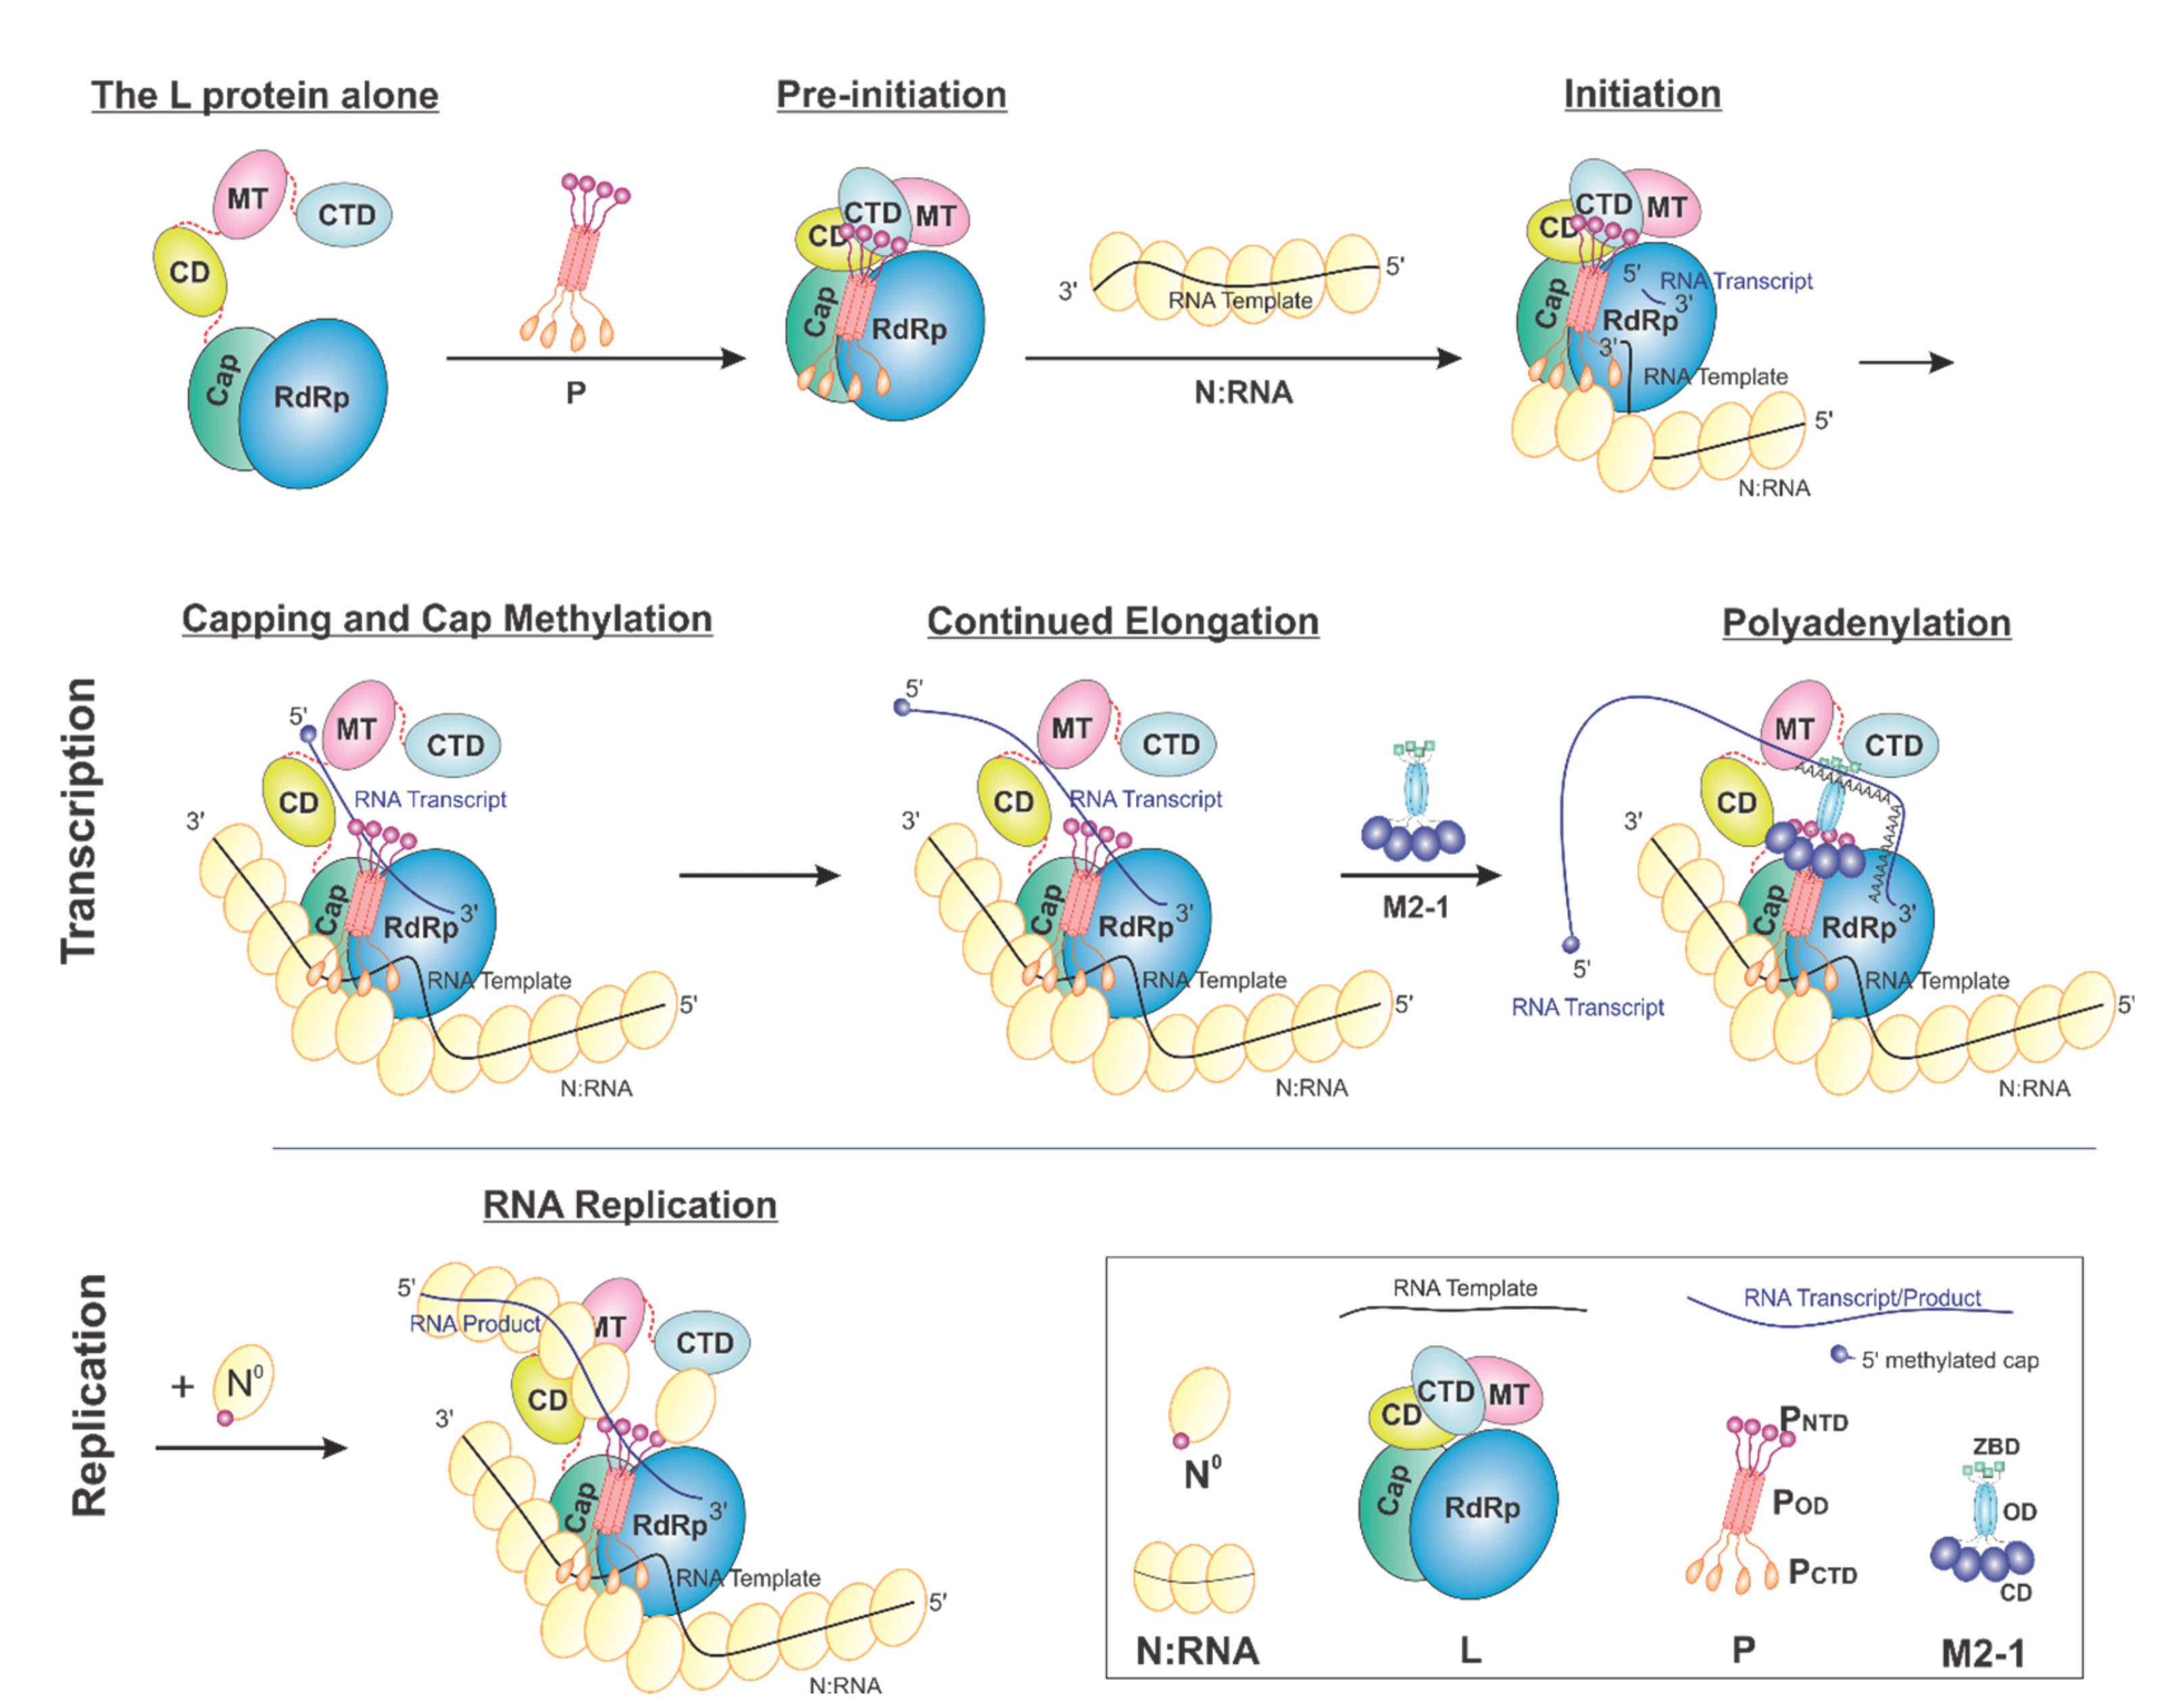
\includegraphics[width=1\linewidth]{04. Introduction//Figs/09. N_p_l_m21-interaction-overview.png}  
    \caption[A Model of RNP-Mediated RSV RNA Transcription and Replication.]{\textbf{A Model of RNP-Mediated RSV RNA Transcription and Replication.} The L protein, composed of the connector domain (CD), the methyltransferase domain (MT), the C-terminal domain (CTD), the Cap domain, and the RdRp domain, undergoes conformational rearrangement after interacting with tetrameric P protein in the pre-initiation step. During the initiation stage, the nucleocapsid, composed of N polymer bound to the RSV RNA template, is recruited by interaction with P protein. This causes a partial liberation of the RNA template and allows L to access it. If the RNA transcription follows, the Cap and the MT domains rearrange to catalyze the cap addition and cap methylation. Afterwards, the elongation stage of the transcription continues until the transcript polyadenylation step, which is mediated by M2-1 recruitment. Upon the supply of the N° (RNA-free N), the RNA replication continues. Figure taken from \cite{Cao2021StructuralComplexes}.}
    \label{fig:A Model of RNP-Mediated RSV RNA Transcription and Replication}
\end{figure}



\subsection{RSV Inclusion Bodies} \label{subsec:RSV Inclusion Bodies}


% talk about assembly and llps and ibags



\begin{figure}
    \centering
    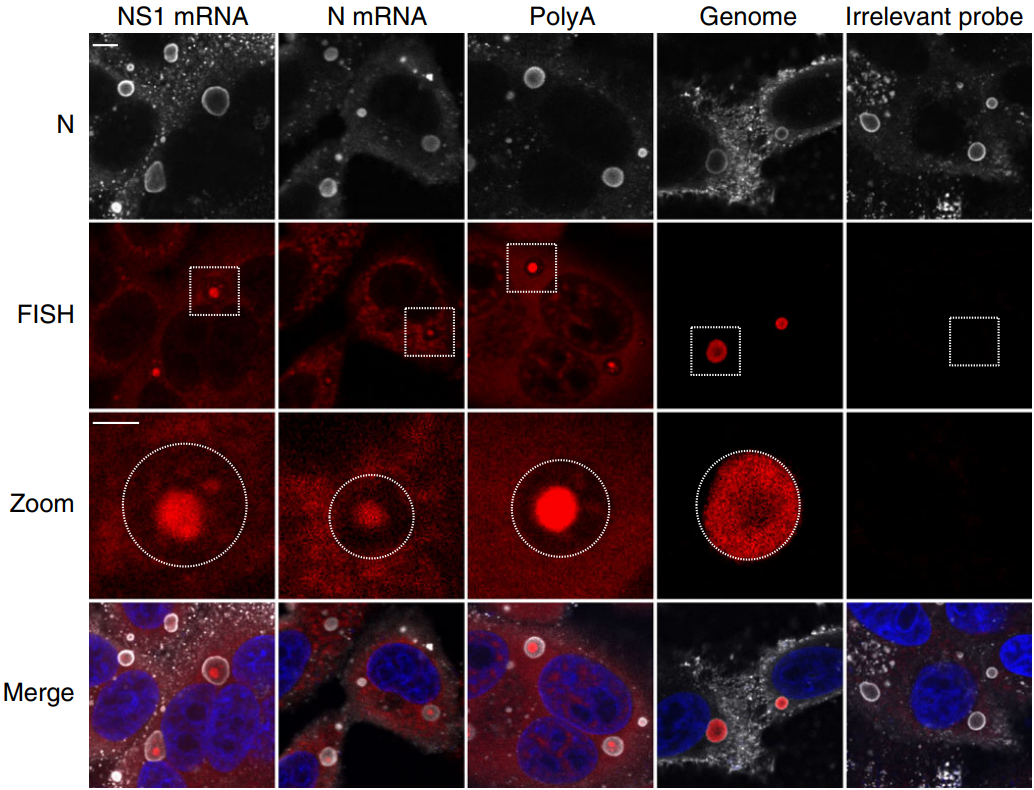
\includegraphics[width=1\linewidth]{04. Introduction/Figs/11. RSV IBs.png}  
    \caption[Viral RNA Discrete Localisation in hRSV Infected Cells.]{\textbf{Viral RNA Discrete Localisation in hRSV Infected Cells.} hRSV-infected HeLa cells were fixed 24 hours post-infection (HPI) and stained for the N protein (inclusion body identification) and specific RNA species using fluorescence \textit{in situ} hybridization (FISH). The latter were NS1 mRNA, N mRNA, polyadenylated RNA (PolyA), and viral genomic RNA which all localised within the inclusion body structures. Circles in the zoom panel represent IB boundaries. The scale bar in the top panel indicates 5 \(\mu\)m, while the one present in the zoom panel is 2 \(\mu\)m. Figure taken from \cite{Rincheval2017FunctionalVirus}.}
    \label{fig:Viral RNA Discrete Localisation in hRSV Infected Cells}
\end{figure}

\subsubsection{Function of RSV IBs} \label{Function of RSV IBs}

IBs are amorphous membranelles aggregates, which have been observed to form as early as 6 hours post-infection and often localise in close proximity to the nucleus (\cite{Bachi1973MorphogenesisVirus}; \cite{Jobe2020RespiratorySignaling}). They have characteristics of biomolecular condensates (with a similar electron density under electron microscopy to the nucleoli) and resemble cytoplasmic inclusions associated with other viral infections e.g. Negri bodies forming during rabies virus infection (\cite{Nikolic2017NegriOrganelles}). RSV N and P proteins are found on the edges of IBs, while L and M2-1 proteins are located inside the structure. (\cite{Rincheval2017FunctionalVirus}), using super-resolution imaging, discovered internal IB compartments called IB-associated granules (IBAGs). These not only contained different viral proteins compared to the rest of the IB, but nascent RNA labelling also suggested IBAGs to be the sites where newly synthesized mRNA concentrates (\cite{Jobe2020RespiratorySignaling}; \cite{Richard2018RSVTranscription}). Taken together, data suggests that IBs are specialised sites which enable viral replication and transcription and that these processes may be compartmentalised.

It is currently unknown if IFIT proteins interact with these structures. Given the well-described roles of IFITs in sensing viral RNA, it is possible that different IFITs may localise into IBs and IBAG, potentially interacting with viral RNA before the capping process takes place or directly interfere with the translational machinery. It is also possible that IFITs are restricted from accessing IBs by an unknown mechanism. Understanding these processes may reveal novel routes of increasing viral sensitivity to the innate immune response.



\cite{Whelan2016FunctionalDisorder} - Functional correlations of respiratory syncytial virus proteins to intrinsic disorder





\section{Aims of the Study} \label{sec:Aims}
Here have a page of the aims.

A detailed comparative study of human and bovine IFITs and their interaction with RSV. Looking at their induction, expression, and changes in localisation. Looking at interaction with RSV IBs. Assessing the involvement of IFIT2 in the RSV life cycle.

For your Aims make sure these are very detailed, so 2 pages roughly. Not 3-4 bullet points of 2 lines each, which I have seen!

clearly human ifits are global restictors of hrsv. but is it relevant, do they get induced? can we isolate what is inducing them if so? 

are human ifits induced by brsv and thus have a potential to crossprotect from it?

does this reproduce in bifit with brsv and crossprotection from hrsv?

through what mechanism are ifits inhibitory? where are they located during infection?

do they interact with parts of rsv stuff?

is there a difference between ifits in interaction with htese structures?

%acronyms
\nomenclature[z-DEM]{DEM}{Untranslated}

\nomenclature[z-IBAG]{IBAG}{IB-Associated Granule}
\nomenclature[z-IB]{IB}{Inclusion Body}
\nomenclature[z-BVDV]{BVDV}{Bovine Viral Diarrhoea Virus}
\nomenclature[z-HCV]{HCV}{Hepatitis C Virus}
\nomenclature[z-TULV]{TULV}{Tula Virus}
\nomenclature[z-PHV]{PHV}{Prospect Hill Virus}
\nomenclature[z-PIV3]{PIV3}{Parainfluenza Virus 3}
\nomenclature[z-STING]{STING}{Stimulator of Interferon Genes}
\nomenclature[z-TBK1]{TBK1}{TANK-Binding Kinase 1}
\nomenclature[z-HEK]{HEK}{Human Embryonic Kidney}
\nomenclature[z-eIF]{eIF}{Eukaryotic Initiation Factor}
\nomenclature[z-ssRNA]{ssRNA}{Single-Stranded RNA}
\nomenclature[z-TPR]{TPR}{Tetratricopeptide Repeat}
\nomenclature[z-IFIT]{IFIT}{Interferon-Induced Protein with Tetratricopeptide Repeats}
\nomenclature[z-ISG]{ISG}{Interferon-Stimulated Gene}
\nomenclature[z-UTR]{UTR}{Untranslated Region}
\nomenclature[z-IRSE]{IRSE}{Interferon-Stimulated Response Elements}
\nomenclature[z-STAT]{STAT}{Signal Transducer and Activator of Transcription}
\nomenclature[z-JAK]{JAK}{Janus Kinase}
\nomenclature[z-IRF]{IRF}{Interferon Regulatory Factor}
\nomenclature[z-ISGF3]{ISGF3}{Interferon-Stimulated Gene Factor 3}
\nomenclature[z-5'-PPP]{5'-PPP}{5'-Triphosphoate}
\nomenclature[z-m7G]{m7G}{7-Methyl Guanosine}
\nomenclature[z-dsRNA]{dsRNA}{Double-Stranded RNA}
\nomenclature[z-MAVS]{MAVS}{Mitochondrial Antiviral Signalling Protein}
\nomenclature[z-RIG-I]{RIG-I}{Retinoic Acid-Inducible Gene I}
\nomenclature[z-MDA5]{MDA5}{Melanoma Differentiation-Associated Gene 5}
\nomenclature[z-NF\(\kappa\)B]{NF\(\kappa\)B}{Nuclear Factor kappa B}
\nomenclature[z-RSV]{RSV}{Respiratory Syncytial Virus}
\nomenclature[z-PRR]{PRR}{Pattern Recognition Receptor}
\nomenclature[z-PAMP]{PAMP}{Pathogen-Associated Molecular Pattern}
\nomenclature[z-LPS]{LPS}{Lipopolysaccharide}
\nomenclature[z-TLR]{TLR}{Toll-Like Receptor}


%Words in text: 2625
%Words in headers: 112